\documentclass[a4paper]{article}

\usepackage[T2A]{fontenc}
\usepackage[russian]{babel}
\usepackage{graphicx}
\usepackage{float}
\usepackage{hyperref}
\usepackage{amsmath, amssymb}
\usepackage{caption}
\usepackage{geometry}
\usepackage{pdfpages}
\geometry{top=2cm,bottom=2cm,left=2cm,right=2cm}

\newcommand{\minus}{\scalebox{0.75}[1.0]{$-$}}



\begin{document}

\begin{center}
\textsc{Санкт-Петербургский национальный исследовательский институт информационных технологий, механики и оптики\\[3mm]
Физический факультет} \\[3mm]

\end{center}
\vspace{5mm}

\vspace{2mm}
\line(1,0){\textwidth}
\vspace{5mm}
\begin{minipage}{0.4\textwidth}
    Группа: Z3144 \\
    Студент: Евгений Турчанин\\
    \vspace{1mm}
\end{minipage}
\hfill
\vspace{1mm}
\line(1,0){\textwidth}


\section{ \textbf{Цели работы}}

Изучение режимов колебаний в простейшей системе двух связанных осцилляторов и сопоставление с элементарной теорией связныхосцилляторов.

\section{\textbf{Задачи}}

\begin{enumerate}
    \item  Измерение частоты синфазной колебательной моды системы.
    \item  Измерение частоты при колебаниях системы в противофазе.
Измерение константы связи и коэффициента жёсткости пружины.
    \item  Измерение периода и частоты биений, возникающих при возбуждении двумодового колебательного процесса.
\end{enumerate}


\section{\textbf{Теоретическое введение}}
Уравнения движения для связных колебаний выглядит как:
\begin{equation}
    \begin{cases}
        \ddot{\varphi_1}+\omega_0^2\varphi_1-\varkappa^2(\varphi_2-\varphi_1)=0\text{,}\\
        \ddot{\varphi_2}+\omega_0^2\varphi_2-\varkappa^2(\varphi_1-\varphi_2)=0\text{.}
    \end{cases}
\end{equation}
Где $\varphi_{1\text{,} 2}$ --- углы отклонения от вертикали 1-го и 2-го маятника соответственно, $\omega_0$ --- собственная частота колебаний без затухания, $\varkappa^2=\dfrac{kL_1^2}{mL_2^2}$, $k$ --- коэффициент жёсткости, $L_{1, 2}$ --- расстояние от крепления до пружины, $m$ --- масса груза.\\
\begin{figure}[H]
    \center
    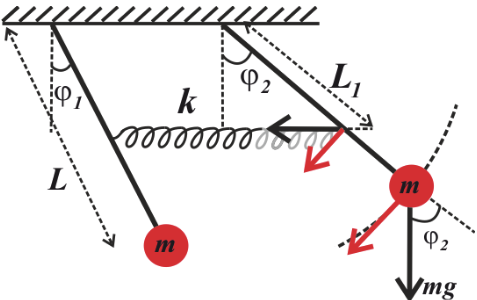
\includegraphics[width=0.5\textwidth]{pick_1.png}
\end{figure}
Решением данной системы:
\begin{equation}
    \begin{cases}
        \varphi_1=\frac{1}{2}(\Phi_{01}\cos(\Omega_{n1}+\varphi_{01}))+\Phi_{02}\cos(\Omega_{n2}+\varphi_{02})\text{,}\\
         \varphi_2=\frac{1}{2}(\Phi_{01}\cos(\Omega_{n1}+\varphi_{01}))-\Phi_{02}\cos(\Omega_{n2}+\varphi_{02})\text{.}
    \end{cases}
\end{equation}
Где $\Phi_{01, 02}$ --- амплитуды 1-го и 2-го соответственно, $\varphi_{01, 02}$ --- начальные фазы 1-го и 2-го соответственно, $\Omega_{n1}=\omega_0$, $\Omega_{n2}=\sqrt{\omega_0^2+2\varkappa^2}$\\
Так как $\varkappa^2/\omega_0^2$ --- это малый параметр, то верно:
\[
    \Omega_{n2}=\sqrt{\omega_0^2+2\varkappa^2} \approx \omega_0\left(1+\dfrac{\varkappa^2}{\omega_0^2}\right)=
    \sqrt{\dfrac{g}{L}}+\dfrac{kL_1^2}{mg^{1/2}L^{3/2}}
\]

\[
    T_{\text{б}}=\dfrac{2\pi}{\Omega_{n2}-\Omega_{n1}}
\]

\section{\textbf{Данные}}
\begin{figure}[H]
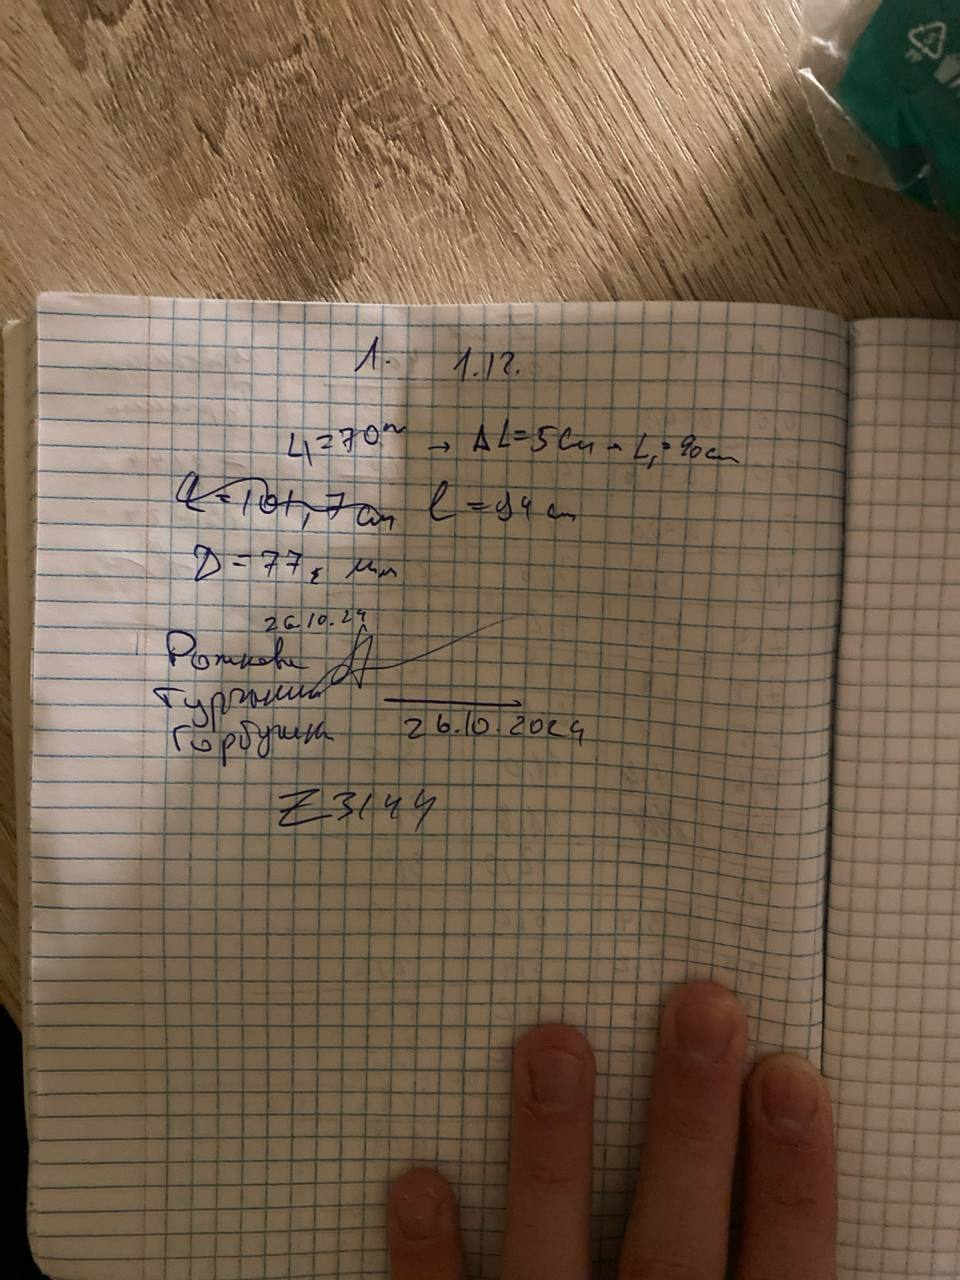
\includegraphics[width=0.5\textwidth]{pick_me}
\end{figure}


\section{\textbf{Результаты}}
Обрабатывая данные в python, получаем:

\begin{figure}[H]
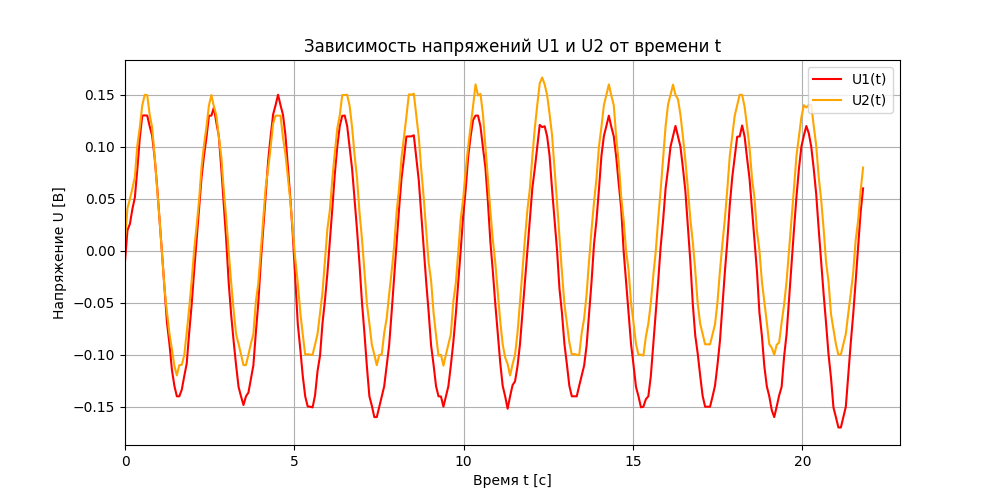
\includegraphics[width=0.5\textwidth]{gra_1}
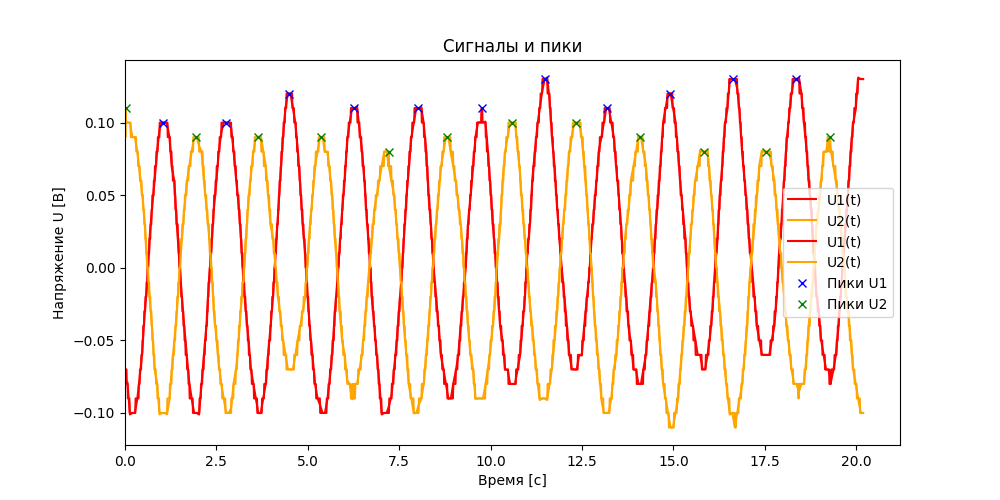
\includegraphics[width=0.5\textwidth]{gra_2}
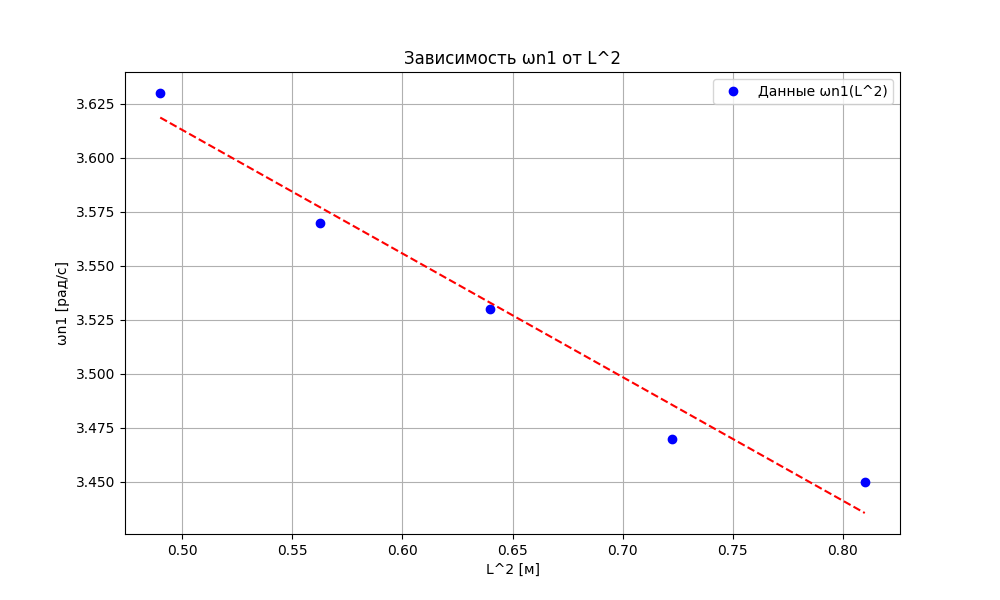
\includegraphics[width=0.5\textwidth]{gra_3}
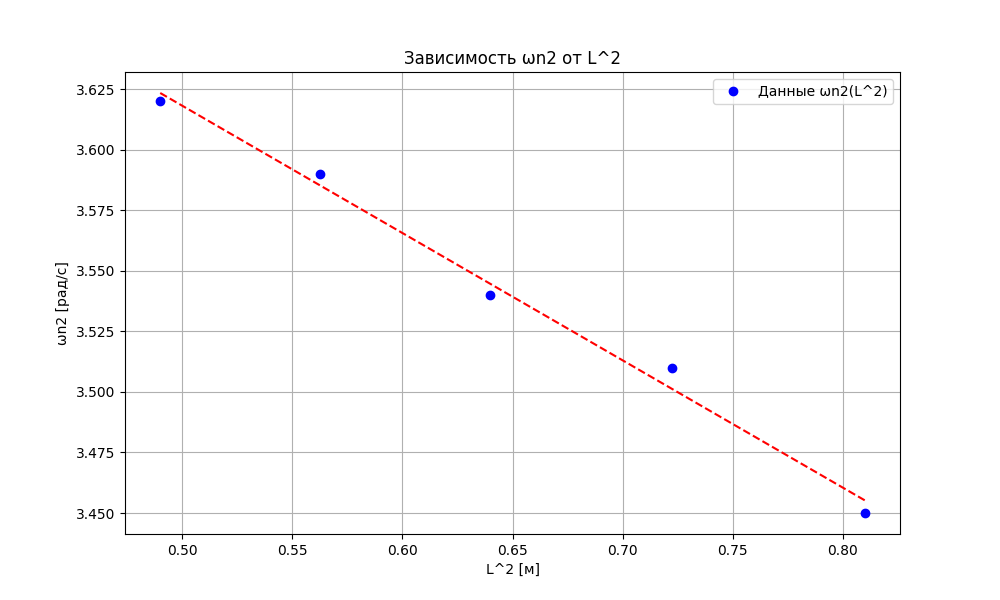
\includegraphics[width=0.5\textwidth]{gra_4}
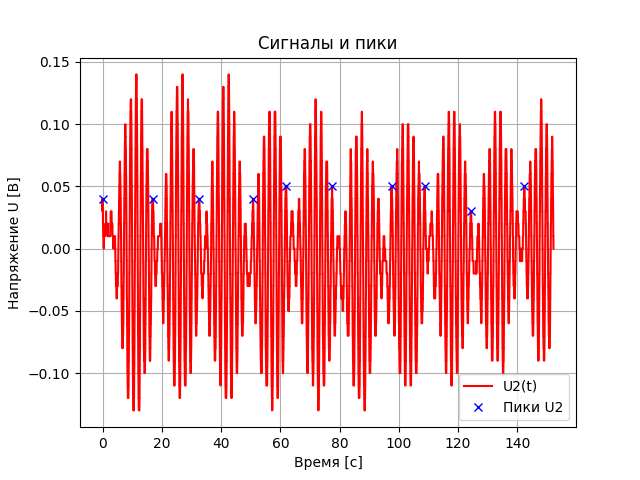
\includegraphics[width=0.5\textwidth]{gra_5}
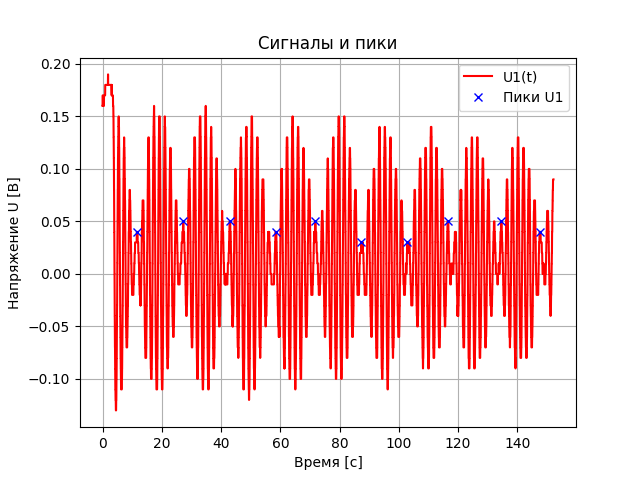
\includegraphics[width=0.5\textwidth]{gra_6}
\end{figure}

\center
\begin{enumerate}
\item
Из графика $\Omega_{n1}$= 3.186, 3.172\\
Теоретическое $\Omega_{n1}$= 3.166
\item
Средний $\Omega_{12}$: $3.63$ c\\
Коэффициент жесткости k: $1.76 \pm 0.058$ $H/m$\\
Коэффициент k: $-0.57 \pm 0.058$\\
\item
Средний $\Omega_{22}$: $3.59$ c \\
Коэффициент k: $-0.53 \pm 0.029$\\
Коэффициент жесткости k: $1.62 \pm 0.029$\\


\item
Доверительный интервал частоты $\Omega_{1}$: $0.42 \pm 0.084$\\
Средний период 1 биений по графику: $15.12$ секунд\\

Доверительный интервал частоты $\Omega_{2}$: $0.40 \pm 0.150$\\
Средний период 2 биений по графику: $15.80$ секунд
\end{enumerate}


\section{\textbf{Вывод}}

\begin{enumerate}
    \item Коэфициет жесткости $k$ получился ровно в два раза меньше, что может быть вызванно ошибкой в вычисления или неправильной обработкой в python
    \item Так же для частоты $\Omega_2$ получился большой доверительный интервал, это может быть вызванно, тем что запуск маятника происходил путем простого отпускания рук, а из-за этого могли сильно отличатся начальные данные
    \item В остальном, теория сходится с экспериментом
\end{enumerate}
\end{document}
